\documentclass[letterpaper,journal]{IEEEtran}
\usepackage[T1]{fontenc}
\usepackage{amsmath,amssymb,amsfonts,amsthm}
\usepackage{array,booktabs,multirow,threeparttable}
\usepackage{algorithm,algorithmic}
\usepackage{graphicx,cite,url}
\usepackage{stfloats}
\usepackage{placeins}
\usepackage[hidelinks]{hyperref}
\graphicspath{{figures/}}
\newcommand{\method}{CFCMT}
\newcommand{\R}{\mathbb{R}}
\newcommand{\ind}{\mathbf{1}}
\DeclareMathOperator*{\argmin}{arg\,min}
\DeclareMathOperator*{\argmax}{arg\,max}
\DeclareMathOperator{\range}{range}
\DeclareMathOperator{\median}{median}
\newtheorem{proposition}{Proposition}
\newtheorem{theorem}{Theorem}
\newtheorem{lemma}{Lemma}
\newtheorem{remark}{Remark}
\hyphenation{net-work net-works coun-ter-fac-tual}
\hypersetup{pdftitle={CFCMT: Cross-City Traffic Signal Control via Matched Action-Cost Prediction and Source Selection},pdfauthor={Yifan Zhang, Liang Zheng, Qifan Zhang, and Haoming Li},pdfsubject={IEEE T-ITS manuscript}}

\begin{document}
\title{CFCMT: Cross-City Traffic Signal Control via\\Matched Action-Cost Prediction and Source Selection}
\author{Yifan~Zhang, Liang~Zheng, Qifan~Zhang, and Haoming~Li%
\thanks{Yifan Zhang (e-mail: erzhu419@gmail.com; 204201048@csu.edu.cn) and Liang Zheng (corresponding author; e-mail: zhengliang@csu.edu.cn) are with the School of Traffic and Transportation Engineering, Central South University, Changsha, Hunan, China.}%
\thanks{Qifan Zhang is with the Faculty of Information Technology, Monash University Malaysia, Malaysia (e-mail: zhangqifan0419@gmail.com).}%
\thanks{Haoming Li is with the Department of Transportation Engineering, School of Ocean and Civil Engineering, Shanghai Jiao Tong University, Shanghai, China (e-mail: lihaoming@sjtu.edu.cn).}}
\markboth{Manuscript prepared for IEEE Transactions on Intelligent Transportation Systems}%
{CFCMT: Cross-City Traffic Signal Control}
\maketitle

% Abstract
\begin{abstract}
Cross-city transfer for urban traffic signal control is complicated by differences in topology, signal phases, and demand. This paper presents Causal-Factored Cross-City Model Transfer, a supervised predeployment framework for matched phase-cost prediction and source selection. Restricted reference and antisymmetric pairwise predictors combine an 18-network source bank in seven groups with target adaptation labels. Eight development seeds select source weights and an error-score guard before deployment. The frozen pipeline is evaluated against six baselines in 1,568 one-hour simulations across four scenarios in Los Angeles and Jinan. The 56 evaluation seeds are disjoint from this selection panel but were used in earlier controller experiments. Mean city-wise relative waiting decreases by 2.42\% against MaxPressure, with a 95\% paired bootstrap interval of 0.66--4.58\% and Holm-adjusted p-value of 0.0082. Against the exact generalized-pressure reference, the mean waiting-time change is $-1.01\%$, with a 95\% interval of $[-3.06,+0.60]\%$. In Jinan, 167 of 168 runs have identical outcomes across all ten recorded metrics. These results describe the complete pipeline on a reused benchmark panel; they do not establish positive incremental benefit over its own reference or control gains attributable to cross-city source data.
\end{abstract}

\begin{IEEEkeywords}
Modelling and simulation, optimization and control, road transportation, traffic networks, traffic signal control, cross-city transfer learning.
\end{IEEEkeywords}

% Introduction
\section{Introduction}
\label{sec:intro}

\IEEEPARstart{A}{daptive} urban traffic signal control (TSC) reduces congestion and vehicular delay. Deep reinforcement learning (DRL) has shown potential in calibrated simulators, but transfer across road networks remains challenging \cite{wei2019presslight,chen2020thousandlights}. Online exploration and intersection-specific reward tuning incur high operational costs. A practical cross-city framework must therefore define its predeployment target information and provide closed-loop operation with fixed controller parameters.

Existing transferable signal control strategies can be broadly categorized into pressure-based heuristics and parameter-shared neural architectures. Specifically, MaxPressure (MP) selects signal phases according to upstream-to-downstream queue differentials and provides theoretical queue stability under the assumptions of the underlying traffic model \cite{varaiya2013maxpressure}. To handle varying intersection geometries, the flipping- and rotation-invariant all-phase (FRAP) architecture models competition among feasible phases \cite{zheng2019frap}, while MPLight integrates FRAP representations with decentralized pressure-based reinforcement learning \cite{chen2020thousandlights}. Despite these structural advances, transferring learned phase rankings across cities still encounters three primary obstacles:
\begin{enumerate}
    \item \textit{Topological and Phasing Heterogeneity:} Signalized intersections across different cities vary widely in approach geometry, turning-lane allocations, and feasible phase configurations, which complicates direct policy transfer across heterogeneous signal plans.
    \item \textit{Cross-City Regime Mismatch:} Variations in arrival demand intensity, downstream link capacity, and phase clearance intervals alter the relative delay consequences of serving competing traffic movements. Consequently, a phase preference learned in one city may become suboptimal in another.
    \item \textit{Unequal Source Compatibility:} Historical data collected from multiple source cities do not contribute equally to a given target corridor. Combining all source models uniformly can retain incompatible source priors and degrade target-domain traffic efficiency.
\end{enumerate}

To address these issues, we propose Causal-Factored Cross-City Model Transfer (CFCMT), a supervised framework for relative phase-cost prediction and predeployment source selection. Restoring identical simulated states and applying alternative phases yields matched phase-cost contrasts. Each source-group component combines a restricted reference predictor with an antisymmetric pairwise predictor. Source data and matched target outcomes support fitting; separate development runs select mixture weights and an execution guard. The frozen controller then evaluates real-time observations through a sparse conflict coordinator and shared physical signal executor.

The main contributions of this study are summarized as follows:
\begin{enumerate}
    \item \textit{Matched Action-Cost Prediction:} We formulate cross-city signal transfer around short-horizon cost contrasts among candidate phases evaluated from identical traffic states, utilizing standardized movement features and pairwise phase comparisons across heterogeneous signal plans.
    \item \textit{Selective Source Integration and Guarded Execution:} We integrate source-group predictors with a target-domain anchor and determine both the source weights and an error-score execution guard using development rollouts before freezing the controller for evaluation.
    \item \textit{Theoretical Properties of Component Ranking:} We establish common-offset invariance, exact ranking recovery from antisymmetric pairwise contrasts, and an upper bound relating component score error to single-step action regret.
    \item \textit{Paired Closed-Loop Evaluation:} Using an 18-network source bank across seven source groups, we evaluate the frozen controller on the Los Angeles and Jinan benchmark networks across four scenarios and 56 paired seeds against six baseline controllers, including the internal generalized-pressure reference.
\end{enumerate}

% Related work
\section{Related Work}
\label{sec:related}

\subsection{Pressure-Based and Learned Traffic Signal Control}
Varaiya \cite{varaiya2013maxpressure} formulated canonical MP and proved queue stability under the underlying traffic model's assumptions. MP requires no site-specific training and provides a structural baseline for adaptive control. In microscopic operations, pressure-based phase requests must still comply with minimum-green, yellow, and all-red intervals.

In parallel, DRL approaches have incorporated domain-specific traffic structures into state representations, reward functions, and multi-intersection coordination. For instance, PressLight embeds pressure definitions into arterial DRL rewards \cite{wei2019presslight}. FRAP captures phase competition symmetry across traffic movements \cite{zheng2019frap}, and MPLight extends FRAP to large-scale decentralized network control \cite{chen2020thousandlights}. Furthermore, CoLight employs graph attention networks to facilitate cooperation among neighboring intersections \cite{wei2019colight}. Inspired by these structured representations, our study evaluates learned phase-cost predictors alongside deterministic pressure policies under an identical physical signal executor.

\subsection{Transferable and Meta-Learning Signal Controllers}
To reduce the training burden on new road networks, several transferable and meta-learning frameworks have been developed. MetaLight adopts gradient-based meta-reinforcement learning to learn a general initialization that adapts more rapidly to new intersections \cite{zang2020metalight}. General Scenario-Agnostic (GESA) reinforcement learning constructs unified state-action interfaces across diverse intersection topologies \cite{jiang2024gesa}, whereas X-Light leverages transformer architectures to extract transferable decision patterns from multi-city trajectories \cite{jiang2024xlight}. More recently, CrossLight combines offline source pretraining with online target fine-tuning \cite{sun2024crosslight}.

Transfer methods differ in how much target data they require and when those data are collected. \method\ uses matched target simulator interventions for fitting and development rollouts for source-weight and guard selection. Parameters and execution rules are then frozen on the reused benchmark panel. Target-anchor and uniform-source comparisons evaluate this complete predeployment pipeline.

\subsection{Factored Mechanisms and Decision-Relevant Prediction}
Causal and factored representation learning seeks to decompose system dynamics into modular components that generalize more reliably across environments \cite{bengio2019meta,scholkopf2021causal,feng2022factored}. In the context of urban signal control, we operationalize this principle through movement-level traffic features and matched counterfactual simulator interventions. Rather than predicting absolute long-horizon returns, the supervised learning task focuses on estimating relative short-horizon cost differences among feasible phases using histogram-based gradient-boosted decision trees \cite{friedman2001greedy,pedregosa2011scikit}.

Specifically, subtracting a reference phase outcome cancels state-dependent baseline congestion shared by all candidate actions, while an antisymmetric pairwise predictor directly models relative advantages between competing phases. In addition, residual- and context-based error diagnostics are constructed to regulate when the learned phase choice overrides the reference pressure policy, accounting for differences in source-domain compatibility during closed-loop execution.

% Problem
\section{Problem Formulation}
\label{sec:problem}
\subsection{Decentralized Phase Selection and Execution}
Consider an urban road network $n$ consisting of multiple signalized intersections. At each discrete control interval of $\Delta t = 10$~s, each signalized intersection observes its local traffic and signal state $s$ and selects a requested green phase $a$ from the feasible phase set $\mathcal A(s)$. The state vector $s$ summarizes approaching queue lengths, vehicle counts, lane occupancies, the currently active phase, elapsed green time, and neighboring signal states. A shared physical signal executor enforces mandatory minimum-green, yellow, and all-red clearance intervals, thereby decoupling high-level phase requests from low-level safety transitions.

During the offline data collection stage, the complete microscopic state of the Simulation of Urban MObility (SUMO) environment can be saved and restored \cite{lopez2018microscopic}. Let $g$ index a saved network snapshot $s_g$ with feasible phase set $\mathcal A_g=\mathcal A(s_g)$, and let $Y_g(a)$ denote the realized short-horizon traffic cost of requesting candidate phase $a$ followed by a fixed continuation policy. We define a matched \emph{action group} as the complete collection of outcomes $\{Y_g(a)\}_{a\in\mathcal A_g}$ obtained by resetting the simulator and signal executors to the exact same state $s_g$ and applying each candidate phase in turn. Fig.~\ref{fig:framework_overview} summarizes offline matched action-label collection and frozen online execution.

\subsection{Predeployment Target Adaptation Setting}
The predeployment information budget comprises source action groups, target topology and demand specifications, matched target action groups for fitting, and eight target development seeds for selection. Training, source selection, and guard calibration precede evaluation. Closed-loop testing uses real-time observations and frozen predictors without lookahead rollouts. Controlled target simulator resets make this a simulation-assisted adaptation setting, as evaluated in Section~\ref{sec:experiments}.

% Method
\section{Methodology: The CFCMT Framework}
\label{sec:method}
As depicted in Fig.~\ref{fig:framework_overview}, \method\ fits source-group components alongside a target anchor, chooses the source mixture and guard profile using development rollouts, and deploys the frozen controller for online phase selection. 

\begin{figure*}[!t]
\centering
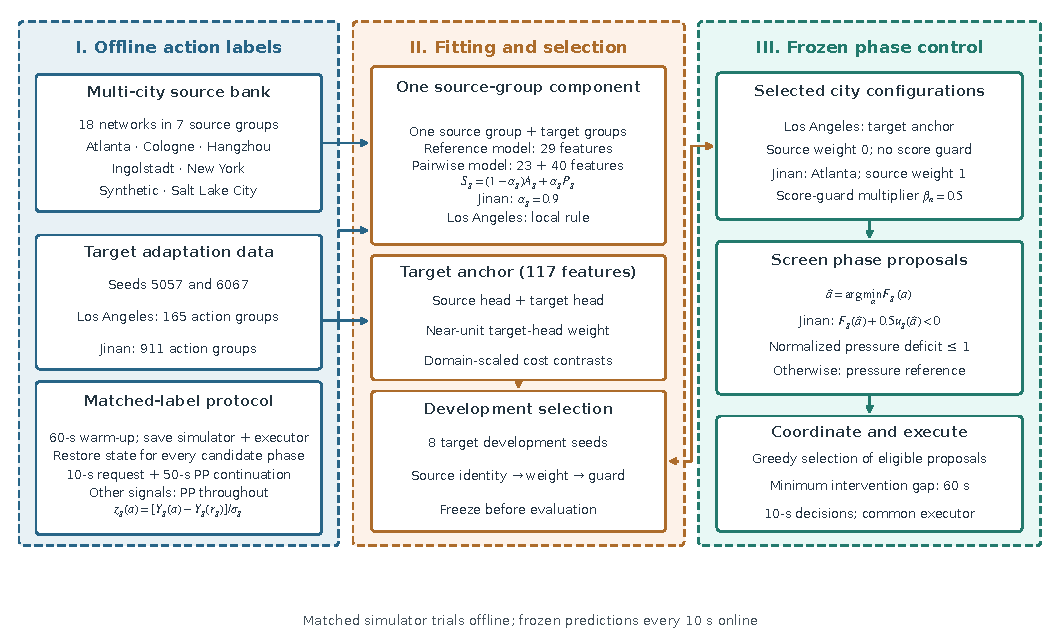
\includegraphics[width=\textwidth]{fig1_framework.pdf}
\caption{Matched action-cost transfer and frozen deployment. Each offline candidate starts from the same restored state, requests a phase for 10~s, and follows PhasePressure (PP) for 50~s. Source components and the target anchor are fitted before eight development seeds select the source weights and guard multiplier. Online decisions use frozen predictions, sparse coordination, and the common executor.}
\label{fig:framework_overview}
\end{figure*}

\subsection{Counterfactual Action-Cost Representation}
After a 60-s warm-up, we save the full microscopic traffic and signal executor states at decision epoch $g$. For each candidate $a\in\mathcal A_g$, the focal intersection requests $a$ for 10~s, then follows PP for 50~s; other intersections follow PP throughout. The branch cost $Y_g(a)$ is the average active and pending vehicle load per controlled incoming lane:
\begin{equation}
 Y_g(a)=\frac{1}{60}\sum_{\tau=1}^{60}
 \frac{N_{\mathrm{active}}(\tau)+N_{\mathrm{pending}}(\tau)}{L_n},
 \label{eq:cost}
\end{equation}
where $\tau \in \{1,\dots,60\}$ indexes the one-second simulation steps within the 60-s evaluation window; $L_n$ denotes the total number of signal-controlled incoming lanes in network $n$; and $N_{\mathrm{active}}(\tau)$ and $N_{\mathrm{pending}}(\tau)$ represent the network-wide numbers of active vehicles and vehicles waiting for network insertion at step $\tau$, respectively. Pending vehicles prevent blocked boundary inflows from appearing as congestion relief. We verify deterministic replay and discard groups with teleports or collisions in any branch, retaining complete feasible-phase outcomes.

To eliminate baseline traffic load variations across snapshots, we anchor phase comparisons against a reference phase $r_g$ selected by a generalized pressure rule. Specifically, for the target networks, $r_g$ maximizes $\Pi_g(a)=q_{\mathrm{green}}(a)-0.02o_{\mathrm{down}}(a)$, where $q_{\mathrm{green}}(a)$ denotes the total queue proxy across incoming lanes served by phase $a$, and downstream occupancy is first averaged over each incoming lane's outgoing lanes. The quantity $o_{\mathrm{down}}(a)$ then averages these values over the incoming lanes served by phase $a$. For each incoming lane $\ell$, the queue proxy is defined as $q_\ell=N_{\mathrm{halted},\ell}+0.35N_{\mathrm{vehicles},\ell}+0.025o_\ell$, where $N_{\mathrm{halted},\ell}$ and $N_{\mathrm{vehicles},\ell}$ denote the numbers of halted and total vehicles on lane $\ell$, and $o_\ell$ is the dimensionless lane occupancy fraction in SUMO. Notice that this reference rule incorporates downstream occupancy, whereas the 50-s PP continuation maximizes $q_{\mathrm{green}}(a)$ alone.

Let $c_g(a)=Y_g(a)-Y_g(r_g)$ denote the cost contrast relative to the reference phase. The normalized training label $z_g(a)$ and the single-step normalized action regret $R_g(\widehat a)$ for a selected phase $\widehat a$ are formulated as:
\begin{align}
 \sigma_g&=\max\{\max_aY_g(a)-\min_aY_g(a),10^{-8}\},\nonumber\\
 z_g(a)&=c_g(a)/\sigma_g,\label{eq:label}\\
 R_g(\widehat a)&=\{Y_g(\widehat a)-\min_aY_g(a)\}/\sigma_g,
 \label{eq:regret}
\end{align}
where $\sigma_g$ is the within-group cost range floored at $10^{-8}$ to prevent division by zero. The implementation also includes a numerical floor equal to $10^{-6}$ times the 75th percentile of $|c_g(a)|$. Since $c_g(r_g)=0$, this additional floor cannot exceed a nonzero group range, giving the equivalent scale in \eqref{eq:label}. Here, $\sigma_g$ is used solely to normalize offline training labels and evaluate offline regret, and is not required during online deployment.

\subsection{Restricted Reference and Pairwise Predictors}
Omitting source-group subscript $k$, each component contains a restricted reference predictor $A_g(a)$ and an antisymmetric pairwise predictor $P_g(a)$.

The reference predictor $A_g(a)=A_\theta(s_g,a)$, with parameters $\theta$, regresses $z_g(a)$ for $a\ne r_g$, fixing $A_g(r_g)=0$. Its 29 features share semantics across networks: aggregate load, queues served or halted by candidate and reference phases, downstream occupancy, phase pressure, switching indicators, clearance intervals, and movement overlap with the active phase. Network identity and raw static geometry are excluded to limit dependence on source-specific layouts. We train histogram-based gradient-boosted regression trees under squared-error loss \cite{friedman2001greedy,pedregosa2011scikit}. Each geographical or synthetic source group (plus the target adaptation set) is treated as a training domain. Sample weights are initialized to balance domains and action groups equally, multiplied by the bounded contrast magnitude $\operatorname{clip}(|z_g(a)|,0.25,4)$, adjusted via capped sign balancing, and normalized to unit mean.

The pairwise predictor uses $x_g\in\R^{23}$ (local congestion, elapsed green, queue concentration, neighboring signal states) and phase descriptor $\phi_g(a)\in\R^{40}$ (served movements, downstream conditions, phase durations, transition overheads). Each unordered phase pair $(a_i,a_j)$ contributes:
\begin{equation}
 \bigl([x_g,\phi_g(a_i)-\phi_g(a_j)],\quad
 t_{gij}=z_g(a_i)-z_g(a_j)\bigr),
 \label{eq:pairdata}
\end{equation}
where $[\cdot,\cdot]$ concatenates vectors and $t_{gij}$ is the empirical cost difference. The reversed pair has target $-t_{gij}$; weights balance domains, action groups, and pairs.

During inference, let $f_\psi$ denote the fitted pairwise tree regressor with parameters $\psi$, and let $\phi_i$ abbreviate $\phi_g(a_i)$. We explicitly enforce antisymmetry on the predicted pairwise cost difference $\widehat\delta_{gij}$:
\begin{equation}
 \widehat\delta_{gij}=\frac{f_\psi(x_g,\phi_i-\phi_j)
 -f_\psi(x_g,\phi_j-\phi_i)}{2}.
 \label{eq:antisym}
\end{equation}
For any decision state with $K_g=|\mathcal A_g|\geq2$ feasible phases, we aggregate the pairwise comparisons into a reference-anchored phase score $P_g(a_i)$:
\begin{align}
 \widetilde P_g(a_i)&=\frac{1}{K_g-1}\sum_{j\ne i}\widehat\delta_{gij},\nonumber\\
 P_g(a_i)&=\widetilde P_g(a_i)-\widetilde P_g(r_g).
 \label{eq:pairscore}
\end{align}
When $K_g=1$, only a single phase is feasible and no scoring is required. Both $A_\theta$ and $f_\psi$ are trained using a learning rate of 0.05, 100 boosting iterations, a maximum of 15 leaves, $L_2$ regularization of 10, and minimum leaf sizes of 12 and 20, respectively.

\subsection{Component Blending and Error Diagnostics}
Within each source-group component, the reference predictor $A_g(a)$ and pairwise predictor $P_g(a)$ are combined via a blending weight $\alpha_g \in [0, 1]$ to yield the component phase score $S_g(a)$:
\begin{equation}
 S_g(a)=(1-\alpha_g)A_g(a)+\alpha_gP_g(a),\qquad
 \widehat a_g=\argmin_{a\in\mathcal A_g}S_g(a),
 \label{eq:blend}
\end{equation}
where Jinan components use $\alpha_g=0.9$. The Los Angeles source candidates and equal-source baseline use the adaptive agreement rule \eqref{eq:la-component-blend} in Appendix~\ref{app:score-proofs}; the final Los Angeles controller selects the target anchor instead.

We construct heuristic error penalties from fitted residuals and differences in static network context. Let $e_A$ and $e_P$ denote the 90th percentiles of absolute in-sample training residuals (floored at $10^{-6}$) for $A_\theta$ and $f_\psi$, respectively, and let $d_g$ denote the Euclidean distance from the static network context to the nearest training-network support context after standardization by domain-centroid spread. For any non-reference phase $a_i \ne r_g$, the predictor error scores $u_{A,g}(a_i)$ and $u_{P,g}(a_i)$ are defined as:
\begin{align}
 u_{A,g}(a_i)&=e_A(1+0.25d_g),\nonumber\\
 v_g(a_i)&=\frac{1}{K_g-1}\sum_{j\ne i}
 \left|\widehat\delta_{gij}-(\widetilde P_g(a_i)-\widetilde P_g(a_j))\right|,\nonumber\\
 u_{P,g}(a_i)&=(e_P+v_g(a_i))(1+0.25d_g),
 \label{eq:error_scores}
\end{align}
with $u_{A,g}(r_g)=u_{P,g}(r_g)=0$. Here, $v_g(a_i)$ measures disagreement between the antisymmetric pairwise predictions $\widehat\delta_{gij}$ and the aggregated score differences $\widetilde P_g(a_i)-\widetilde P_g(a_j)$. It includes the aggregation scale factor in \eqref{eq:recovery} and can therefore remain positive even for exact pairwise predictions. These quantities are heuristic error diagnostics rather than calibrated probability intervals. Restoring the source-group index $k$, the combined error score for component $k$ is given by $u_{k,g}(a)=(1-\alpha_g)u_{A,g}(a)+\alpha_gu_{P,g}(a)$.

\subsection{Source Selection and Guarded Execution}
\label{sec:source-selector}
Let $\mathcal K$ index the seven source groups. Each component $S_{k,g}(a)$ pools source group $k$ with the target adaptation groups. The target anchor $T_g(a)$ instead interpolates two 117-feature heads: a source head fitted on the complete source bank, excluding target examples, and a target head fitted only on the target adaptation groups. Each head divides contrasts by its training domain's median positive action-group range, applies a numerical floor, and clips labels to $[-5,5]$. Both use squared-error trees with learning rate 0.05 and no early stopping. The source head uses 100 iterations, 15 leaves, minimum leaf size 12, and $L_2$ penalty 10; the target head uses 80, 7, 4, and 16, respectively. With prior strength zero and cap one, the target interpolation weight is $\eta_n=N_{T,n}/(N_{T,n}+10^{-12})$, where $N_{T,n}$ counts target action groups. For 165 Los Angeles and 911 Jinan groups, the implemented floating-point source weights $1-\eta_n$ are approximately $6.0\times10^{-15}$ and $1.1\times10^{-15}$. Ordinary score interpolation lets this tiny source term affect equal or nearly equal target predictions.

Given non-negative source mixture weights $\{\omega_{n,k}\}_{k\in\mathcal K}$ satisfying $\sum_{k\in\mathcal K}\omega_{n,k}\leq1$ for target network $n$, the ensemble cost score $F_g(a)$ blends the target anchor with the source-group components:
\begin{equation}
 \begin{split}
 F_g(a)={}&\left(1-\sum_{k\in\mathcal K}\omega_{n,k}\right)T_g(a)\\
 &+\sum_{k\in\mathcal K}\omega_{n,k}S_{k,g}(a).
 \end{split}
 \label{eq:source-mixture}
\end{equation}
Similarly, the ensemble error diagnostic $u_g(a)$ is computed using the same convex combination of the anchor error score and component error scores $\{u_{k,g}(a)\}_{k\in\mathcal K}$. Each anchor head uses the residual/context error rule in the first line of \eqref{eq:error_scores}, computed from its own fitted data. The anchor error interpolates its source and target head errors with target weight $\eta_n$ and adds their absolute score difference multiplied by the product of the two interpolation weights. The source weights $\omega_{n,k}$ are distinct from the within-component blend $\alpha_g$.

Eight separate development seeds determine the source weights $\omega_{n,k}$ and guard multiplier $\beta_n$. Against the target anchor, eligible source and weight candidates must improve mean seed-wise relative waiting by at least 0.5\%, limit worst-seed regression to 1.0\%, and add no collision or teleport incidents on any seed. Their waiting score is the mean relative change plus half its population standard deviation and the positive part of the worst change. Selection proceeds in three stages:
\begin{enumerate}
    \item \textit{Source Identity Profiling:} Each source group is screened at weight 0.75. The eligible source with the lowest waiting score is selected; otherwise, the anchor is retained.
    \item \textit{Source Weight Selection:} The selected source is tested at weights $\{0,0.25,0.5,0.75,1\}$. The lowest-scoring eligible positive weight is selected; otherwise, the anchor is retained.
    \item \textit{Execution Guard Calibration:} Guard multipliers $\beta_n\in\{0,0.25,0.5\}$ are compared with the selected unguarded controller. The aggregate numbers of collision incidents and teleports must each not increase, and worst-seed waiting regression must not exceed 1.0\%. Eligibility additionally requires a decrease in either incident count or at least 0.5\% mean relative waiting improvement. Eligible guards minimize combined incidents, then the waiting score; otherwise, the unguarded controller is retained.
\end{enumerate}

Following this protocol, for the Jinan network, the procedure selects the Atlanta source component with $\omega_{n,\mathrm{Atlanta}}=1$ and guard multiplier $\beta_n=0.5$. Let $\widehat a=\argmin_aF_g(a)$ denote the lowest-cost candidate phase. Under the execution guard, a departure $\widehat a\ne r_g$ is eligible to replace the reference phase only if both an error-penalized improvement condition and a normalized pressure-deficit bound are satisfied:
\begin{equation}
 \begin{gathered}
 F_g(\widehat a)+\beta_nu_g(\widehat a)<0,\\
 \frac{\max\{\Pi_g(r_g)-\Pi_g(\widehat a),0\}}
 {\max\{|\Pi_g(r_g)|,1\}}\leq1.
 \end{gathered}
 \label{eq:execution-guard}
\end{equation}
Failing \eqref{eq:execution-guard} returns the pressure reference $r_g$; passing it submits a proposal that still requires coordinator approval. Los Angeles retains the unguarded target anchor because all single-source candidates increase development waiting time; its proposals also pass through the coordinator.

The sparse coordinator connects two signals if their incoming-plus-immediate-outgoing lane neighborhoods overlap, or if either is the other's next downstream signal in the routing graph. Proposals are ranked by descending priority $\max\{-F_g(\widehat a),0\}$ without the guard and $\max\{-F_g(\widehat a)-\beta_nu_g(\widehat a),0\}$ with it; ties use lexicographic signal identifiers. Greedy admission excludes conflicts with already admitted signals. A positive cooldown counter at a signal or conflicting neighbor blocks its proposal. After each decision, existing counters decrease by one and admitted signals receive counter five. This blocks five intervening 10-s decision epochs, giving a minimum 60-s intervention gap at the same or conflicting signals. Only admitted learned requests reach the physical executor; other signals request $r_g$.

\subsection{Theoretical Properties of Component Scores}
Appendix~\ref{app:score-proofs} proves the following matched-contrast and component-ranking properties.

\begin{proposition}[Common-Offset Invariance]
\label{prop:offset}
Suppose the branch cost decomposes as $Y_g(a)=b_g+\mu_g(a)+e_g(a)$, where $b_g$ is a state-dependent baseline offset common to all candidate phases, $\mu_g(a)$ is the true action-dependent cost, and $e_g(a)$ denotes action-dependent estimation noise. Then the cost contrast relative to $r_g$ satisfies:
\begin{equation}
 c_g(a)=\mu_g(a)-\mu_g(r_g)+e_g(a)-e_g(r_g).
 \label{eq:cancellation}
\end{equation}
Consequently, $c_g(a)$ and the induced phase ordering are invariant to arbitrary additive state offsets $b_g$, and $z_g(a)$ is invariant to positive rescaling whenever the numerical floor in $\sigma_g$ is inactive both before and after rescaling.
\end{proposition}

\begin{proposition}[Exact Ranking Recovery from Pairwise Contrasts]
\label{prop:pair-recovery}
The antisymmetric predictor in \eqref{eq:antisym} satisfies $\widehat\delta_{gij} = -\widehat\delta_{gji}$. Moreover, whenever the pairwise predictions are exact ($\widehat\delta_{gij} = z_g(a_i) - z_g(a_j)$ for all $i,j$), the aggregated pairwise score in \eqref{eq:pairscore} satisfies:
\begin{equation}
 P_g(a_i)=\frac{K_g}{K_g-1}\{z_g(a_i)-z_g(r_g)\},
 \label{eq:recovery}
\end{equation}
which strictly preserves the true cost ordering of $z_g(a)$ across all feasible phases $a_i \in \mathcal A_g$.
\end{proposition}

\begin{proposition}[Single-Step Action Regret Bound]
\label{prop:regret_bound}
For the normalized action regret $R_g(\widehat a_g)$ defined in \eqref{eq:regret} and the component phase selection $\widehat a_g = \argmin_{a\in\mathcal A_g} S_g(a)$ in \eqref{eq:blend}, the single-step regret is upper-bounded by:
\begin{equation}
 R_g(\widehat a_g)=z_g(\widehat a_g)-\min_a z_g(a)
 \leq2\|S_g-z_g\|_\infty,
 \label{eq:score-regret-bound}
\end{equation}
where $\|S_g-z_g\|_\infty = \max_{a\in\mathcal A_g}|S_g(a)-z_g(a)|$ denotes the supremum norm error over feasible phases.
\end{proposition}

% Experiments
\section{Experimental Evaluation}
\label{sec:experiments}

\subsection{Multi-City Benchmark and Simulation Setup}
We use SUMO 1.22.0 via \texttt{libsumo} \cite{lopez2018microscopic}, with 18 source networks and two external targets, Los Angeles and Jinan. The source bank contains 317 signals and 6,076 non-internal lanes in seven groups: Atlanta, Cologne, Hangzhou, Ingolstadt, New York, Salt Lake City, and synthetic arterial/grid networks, compiled from the Reinforcement Signal Control (RESCO) and LibSignal benchmarks \cite{ault2021reinforcement,mei2022libsignal}.

Los Angeles is a four-intersection LibSignal arterial; Jinan is a 12-intersection CoLight grid with three demand profiles \cite{wei2019colight}, giving four scenarios. CityFlow networks \cite{zhang2019cityflow} were converted to SUMO while preserving turning movements, phase sequences, and right-of-way rules (Table~\ref{tab:hyperparams}).

\begin{table}[!t]
\centering
\caption{Summary of Simulation and Evaluation Parameters}
\label{tab:hyperparams}
\begin{tabular}{@{}lp{0.53\columnwidth}@{}}
\toprule
Parameter & Value\\
\midrule
Simulation horizon & 3,600 s (including 60-s initialization warm-up)\\
Control decision interval & $\Delta t = 10$ s\\
Counterfactual label horizon & 60 s (10-s candidate phase + 50-s PP)\\
Target adaptation dataset & 2 seeds (165 Los Angeles and 911 Jinan groups)\\
Development selection set & 8 seeds for this selection round\\
Reused-panel evaluation & 56 paired seeds across 7 controllers\\
Total evaluation budget & 1,568 one-hour microscopic simulation runs\\
\bottomrule
\end{tabular}
\end{table}

\subsection{Predeployment Adaptation and Evaluation Protocol}
Offline source action groups are generated using simulation seeds 2027, 3037, and 4047, while target adaptation datasets are collected using seeds 5057 and 6067, yielding 165 matched action groups in Los Angeles and 911 groups in Jinan. Eight development seeds then supply additional closed-loop outcomes for the three-stage selection in Section~\ref{sec:source-selector}, beyond adaptation labels. The selected controllers are the unguarded Los Angeles target anchor and guarded Jinan Atlanta component ($\omega_{n,\mathrm{Atlanta}}=1, \alpha_g=0.9, \beta_n=0.5$).

The eight selection seeds and 56 evaluation seeds are disjoint in this round. Their union is the earlier 64-seed benchmark panel, whose controller results predate this selection round. Evaluation therefore reuses benchmark realizations; all model parameters and execution settings remain frozen. The initial five-controller comparison comprises 1,120 runs. MP and the exact generalized-pressure reference are subsequently added as fixed baseline arms on the same panel, contributing 224 runs each without refitting or parameter selection, for 1,568 runs in total.

\subsection{Compared Baselines and Shared Signal Executor}
We benchmark the frozen \method\ controller against six baselines:
\begin{enumerate}
    \item \textit{Target Anchor (all source weights zero):} The target-dominated predictor without additional source-group components in the deployment mixture. It retains the small source-prior contribution described in Section~\ref{sec:source-selector}.
    \item \textit{Equal Source Weights:} An unselective transfer baseline that assigns uniform weight ($\omega_{n,k}=1/7$) to all seven source-group components under the same city-specific guard and coordinator.
    \item \textit{Dense Linear Residual:} A domain-balanced Huber-ridge regression model ($L_2$ penalty 3, Huber threshold 1.5) fitted to predict residual cost corrections from the full unfactored state and context vector.
    \item \textit{PhasePressure (PP):} An actuated heuristic that greedily selects the phase maximizing approaching queue proxy $q_{\mathrm{green}}(a)$.
    \item \textit{MaxPressure (MP) \cite{varaiya2013maxpressure}:} The implemented pressure controller that maximizes upstream queue proxy minus downstream queue proxy.
    \item \textit{Exact Generalized-Pressure Reference (GP):} Directly requests $r_g$ using the same $\Pi_g$, ordered feasible phases, first-maximum tie rule, warm-up policy, and physical executor as \method, without learned overrides.
\end{enumerate}

All seven controllers operate over the same road networks, demand profiles, 10-s decision epochs, and physical signal executor. Minimum green times follow the positive signal-program specifications; otherwise, the fallback is bounded between 1 and 5~s by the phase duration. Yellow and all-red durations use the corresponding program medians, defaulting to 3~s and 1~s when unspecified, with dynamic 1-s all-red extensions whenever the intersection box remains occupied. Learned controllers additionally use the city-specific guard settings and sparse coordinator; PP, MP, and GP directly request their highest-scoring feasible phases through the shared executor.

\subsection{Evaluation Metrics and Statistical Testing}
The primary metric is mean waiting time (seconds) across all departed vehicles, including unfinished trips at 3,600~s. Waiting and cumulative departures/arrivals include warm-up. System vehicle-hours sum active plus pending vehicle-seconds over $[60,3600]$~s, divided by 3,600. Completion divides cumulative arrivals by departures plus vehicles pending insertion at the endpoint. Vehicles that never depart enter these load/completion measures but not mean waiting. Collision events sum collision records returned by SUMO at each simulation step; incidents deduplicate records with the same vehicle pair, collision type, and lane within each run. Teleport starts and ends are counted separately as simulator diagnostics.

To aggregate results across the two target cities without biasing toward the higher absolute delay in Los Angeles, we first average the three Jinan demand scenarios within each seed, compute the relative waiting-time change $(\text{Wait}_{\method} - \text{Wait}_{\mathrm{base}}) / \text{Wait}_{\mathrm{base}}$ within each city and seed, and then average equally across the two cities and 56 seeds. This mean of city-wise ratios differs from a relative change computed from pooled waiting means. We compute 95\% confidence intervals (CIs) using 20,000 paired seed-level bootstrap resamples and assess statistical significance via two-sided paired Wilcoxon signed-rank tests with Holm step-down multiple-testing correction across the 18 comparator-scope pairs (six comparators and three scopes). Favorable-seed counts refer to negative equal-city averages of the city-wise relative changes. The intervals and tests describe effects on this reused panel, rather than a confirmation independent of the full development history.

% Results
\subsection{Overall Closed-Loop Performance}
\method\ has the best equal-city performance means in Table~\ref{tab:main_results}. Its paired relative waiting change against MP is $-2.42\%$ (95\% CI: $[-4.58,-0.66]\%$; Holm-adjusted $p=0.0082$), favorable in 40 of 56 seeds (Table~\ref{tab:paired_effects}).

\begin{table*}[!t]
\centering
\caption{Closed-Loop Control Performance Across Four Target Scenarios and 56 Paired Seeds}
\label{tab:main_results}
\setlength{\tabcolsep}{4pt}
\begin{tabular}{lrrrrrrr}
\toprule
& \multicolumn{3}{c}{Mean waiting time (s) $\downarrow$} & System & Demand & Collisions & Teleports\\
\cmidrule(lr){2-4}
Controller & Los Angeles & Jinan & \shortstack{Equal-city\\mean} & \shortstack{Vehicle-\\hours $\downarrow$} & \shortstack{Completion\\$\uparrow$} & \shortstack{Events/\\incidents} & \shortstack{Starts/\\ends}\\
\midrule
\method\ (Proposed) & 201.68 & 89.64 & \textbf{145.66} & \textbf{585.42} & \textbf{0.8950} & 26/13 & 0/0\\
Target anchor & 201.68 & 93.97 & 147.83 & 588.48 & 0.8942 & 28/14 & 0/0\\
Equal source weights & 212.45 & 89.62 & 151.03 & 586.27 & 0.8947 & 36/17 & 0/0\\
Dense linear residual & 211.73 & 104.59 & 158.16 & 613.28 & 0.8756 & 41/19 & 0/0\\
PhasePressure (PP) & 231.36 & 89.73 & 160.55 & 600.47 & 0.8778 & 39/19 & 0/0\\
MaxPressure (MP) & 221.49 & 91.57 & 156.53 & 604.78 & 0.8792 & 36/18 & 0/0\\
Exact GP reference & 215.97 & 89.63 & 152.80 & 595.81 & 0.8836 & 41/20 & 0/0\\
\bottomrule
\end{tabular}
\vspace{3pt}
\begin{minipage}{\textwidth}\footnotesize
Note: Each controller row summarizes 224 one-hour simulation runs (4 scenarios $\times$ 56 seeds). Jinan's three demand scenarios are averaged within each seed before equal-city aggregation. Bold identifies the best equal-city performance means; completion is a fraction. Collision events/incidents and teleport starts/ends are unweighted totals over the 224 runs.
\end{minipage}
\end{table*}

The PP interval crosses zero; all three learning-baseline intervals lie below zero (Table~\ref{tab:paired_effects}). \method\ matches the anchor in Los Angeles and improves Jinan waiting by 4.60\%. Equal source weights have a slightly lower Jinan mean (89.62 versus 89.64~s), with 52 of 56 exact city-seed ties.

An effective override in the execution audit is an accepted non-reference switch request or an effective hold of the current green. Los Angeles records 2,123 such overrides in 79,296 decisions (2.6773\%): 322 accepted switch requests and 1,801 holds. In Jinan, one of 713,664 decisions is an accepted switch request; the guard rejects 129,252 of 129,253 model-reference disagreements. Equal source weights admit four Jinan overrides and the anchor 29,359. Supplementary Table~S1 reports the complete agreement, rejection, and override counts and rates for all learned controllers. The selected Jinan policy therefore almost always follows the generalized-pressure reference.

Against GP, the mean paired relative waiting change is $-1.01\%$ (95\% CI: $[-3.06,0.60]\%$; Holm-adjusted $p=1$), favorable in 33 of 56 seeds. The Los Angeles change is $-2.02\%$ (CI: $[-6.13,1.17]\%$); Jinan is $+0.0129\%$ (CI: $[0,0.0386]\%$). These comparisons do not establish a positive incremental waiting-time benefit over GP.

In Jinan, 167 of 168 runs match GP exactly across all ten recorded metrics. The remaining original-demand run (seed 5622039) contains the sole accepted non-reference switch request at 1,880~s. Its pre-request green state matches the GP trace; waiting is 94.01~s under \method\ versus 92.08~s under GP. Vehicle-hours increase by 3.63, while completion rises by 0.540 percentage points. The archived paired records and request traces document this trade-off.

\begin{table}[!t]
\centering
\caption{Paired City-Wise Relative Waiting-Time Changes}
\label{tab:paired_effects}
\setlength{\tabcolsep}{2.5pt}
\begin{tabular}{@{}lrrr@{}}
\toprule
Baseline Comparator & Mean Change (\%) & \shortstack[r]{95\% Bootstrap\\CI (\%)} & \shortstack[r]{Favorable\\Seeds}\\
\midrule
Target anchor & $-2.30$ & $[-2.43,-2.16]$ & 56/56\\
Equal source weights & $-2.46$ & $[-3.15,-1.76]$ & 48/56\\
Dense linear residual & $-9.40$ & $[-10.21,-8.62]$ & 56/56\\
PhasePressure (PP) & $-1.91$ & $[-4.42,0.08]$ & 34/56\\
MaxPressure (MP) & $-2.42$ & $[-4.58,-0.66]$ & 40/56\\
Exact GP reference & $-1.01$ & $[-3.06,0.60]$ & 33/56\\
\bottomrule
\end{tabular}
\vspace{3pt}
\begin{minipage}{\columnwidth}\footnotesize
Note: Relative changes are computed as $(\text{Wait}_{\method}-\text{Wait}_{\mathrm{base}})/\text{Wait}_{\mathrm{base}}$ within each city and seed, then averaged equally across cities and seeds. Negative values indicate waiting-time reductions. Favorable seeds have a negative equal-city mean relative change.
\end{minipage}
\end{table}

\subsection{Analysis of Source Identity and Weight Selection}
Fig.~\ref{fig:source_selection}(a)--(b) compares weight-0.75 source candidates with the anchor on eight development seeds. All seven sources increase Los Angeles waiting by 2.22--7.93\%, so the anchor is retained. Atlanta gives the largest Jinan reduction (0.95\%) and proceeds to weight selection. Across weights $\omega_{n,\mathrm{Atlanta}}\in\{0,0.25,0.5,0.75,1\}$, Jinan waiting is 96.46, 96.26, 96.38, 95.54, and 94.89~s [Fig.~\ref{fig:source_selection}(c)]; unit weight is selected before guard calibration.

\begin{figure*}[!t]
\centering
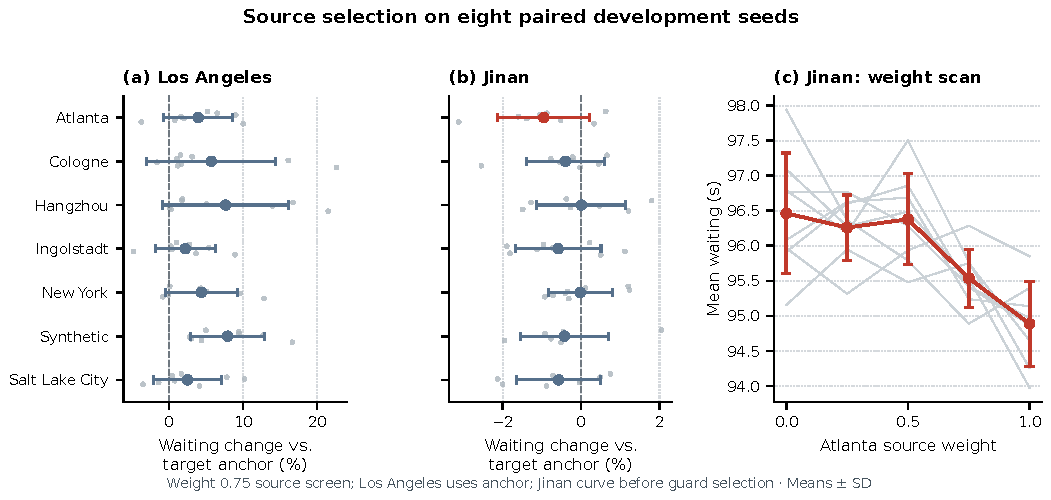
\includegraphics[width=\textwidth]{fig2_source_selection.pdf}
\caption{Source selection on eight development seeds. (a)--(b) Weight-0.75 comparisons with the target anchor; dots denote seeds and bars mean $\pm$ sample standard deviation (SD). (c) Jinan Atlanta-weight scan before guard calibration.}
\label{fig:source_selection}
\end{figure*}

\subsection{Waiting-Time Distributions Across Target Scenarios}
Fig.~\ref{fig:confirmation_distributions} shows run-mean waiting distributions. Los Angeles has a wider range (logarithmic axis), with lower extreme means for \method\ and the anchor than for PP and MP. In Jinan, \method\ has lower medians than the anchor and dense residual baseline, and lies close to PP and equal source weights.

\begin{figure*}[!t]
\centering
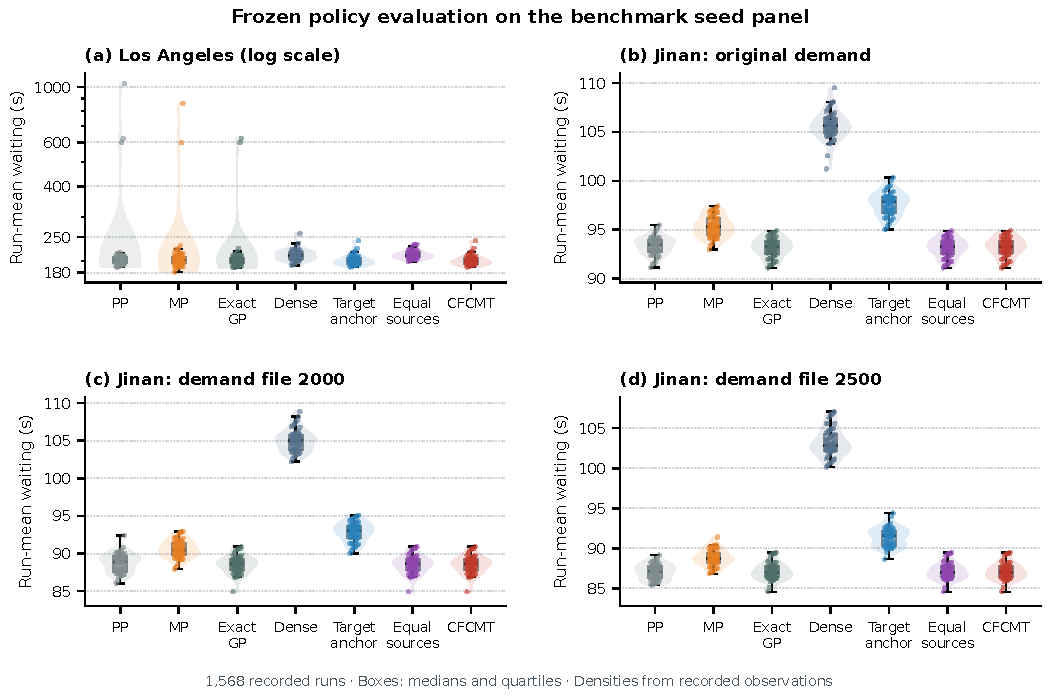
\includegraphics[width=\textwidth]{fig3_benchmark_distributions.pdf}
\caption{Run-mean waiting across four scenarios and 56 reused seeds (1,568 runs). GP: exact generalized-pressure reference. Dots: run means; boxes: medians/quartiles; violins: kernel densities. Los Angeles uses a logarithmic axis.}
\label{fig:confirmation_distributions}
\end{figure*}

\subsection{Effect of the Error-Score Execution Guard}
In Fig.~\ref{fig:guard_comparison}, Jinan waiting is 94.89~s without the guard or at $\beta_n=0$, 89.85~s at 0.25, and 89.60~s at 0.5. The selected $\beta_n=0.5$ gives a 5.57\% mean paired reduction across all eight development seeds. In Los Angeles, $\beta_n=0.5$ lowers mean paired waiting by 1.11\% but raises the worst seed by 4.16\%, exceeding the 1\% regression limit; the unguarded anchor is retained.

\begin{figure*}[!t]
\centering
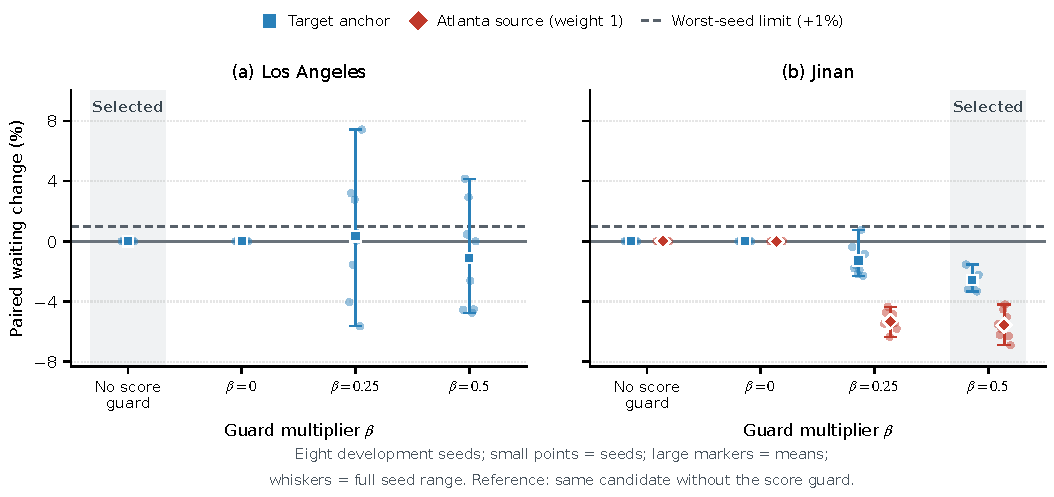
\includegraphics[width=0.99\textwidth]{fig4_guard_comparison.pdf}
\caption{Guard comparison on eight development seeds. Dots denote seeds, large markers mean paired waiting changes, and whiskers the seed range. The dashed line marks the 1\% worst-seed regression limit; shading marks selected configurations.}
\label{fig:guard_comparison}
\end{figure*}

\FloatBarrier

% Discussion
\section{Discussion}
\label{sec:discussion}

\subsection{Selective Transfer Across Heterogeneous Networks}
Los Angeles rejects all seven source groups during development and retains the target anchor (201.68~s versus 212.45~s with equal source weights; Table~\ref{tab:main_results}). Jinan selects the guarded Atlanta component (89.64~s versus 93.97~s for the anchor), while almost always following the reference. These outcomes compare selected pipelines rather than isolate source-data benefits.

\subsection{Short-Horizon Contrasts Versus Closed-Loop Control}
Offline labels measure 60-s active-plus-pending vehicle loads after a 10-s intervention and 50-s PP continuation; evaluation measures waiting accrued by the one-hour endpoint under repeated multi-intersection control. Propositions~\ref{prop:offset}--\ref{prop:regret_bound} concern offset invariance and single-step component regret. The guard \eqref{eq:execution-guard} and coordinator further restrict execution, so full-hour outcomes evaluate the combined procedure.

\subsection{Scope and Limitations}
The anchor and source components differ in feature dimensions, tree capacities, and label normalizations; gains therefore concern the complete selection pipeline. Convex score mixing is assessed empirically. The exact-reference comparison does not establish a positive incremental benefit from learned interventions. Los Angeles selects the target anchor; the selected Jinan source component almost always follows GP. Thus, the present comparisons do not establish control gains attributable to cross-city source data. The 56 reused seeds cover only two target geometries. The aggregate MP comparison is favorable, but the Los Angeles MP interval and aggregate PP interval cross zero. Adaptation requires matched simulator interventions and closed-loop development runs beyond passive field logs. Capacity-matched comparisons, modern published transfer controllers under matched information and execution, and additional cities and data sources remain necessary to assess broader transfer benefits. Supplementary Fig.~S1 retains the smallest-seed Los Angeles departure-cohort example, including unfinished trips and shorter observation windows for later departures.

% Conclusion
\section{Conclusion}
\label{sec:conclusion}
This paper developed \method\ for matched phase-cost prediction and predeployment source selection, combining reference and pairwise predictors, an error-score guard, and sparse coordination. Across 1,568 one-hour Los Angeles and Jinan simulations, mean city-wise relative waiting decreases by 2.42\% against MP, 2.30\% against the target anchor, and 9.40\% against the dense linear residual baseline. On this reused panel, the MP comparison is favorable, while the PP and exact-reference intervals cross zero. Positive incremental benefit over the internal reference and control gains from cross-city source data remain unestablished. Future work concerns capacity-matched architectures, broader target networks, and passive field data.

\section*{Data and Code Availability}
\begingroup\raggedright
The original code and experiment records are available at \href{https://github.com/erzhu419/CFCMT/tree/12e7955d0350e4cac2a344d04954cfb5efea70a2}{GitHub commit \texttt{12e7955}}. The accompanying source archive, version CFCMT-V93-ExactReference-20261031, contains the new 224-run records, per-run execution counts, request traces, analysis and figure scripts, and Supplementary Fig.~S1 and Table~S1. Benchmark networks and demand files retain their upstream licenses.
\par\endgroup

\section*{Acknowledgment}
Google Gemini assisted with initial drafts of the Abstract, Sections~I--VII, and figure layouts. OpenAI ChatGPT and Codex assisted with revisions to those sections and Appendix~\ref{app:score-proofs}. They also assisted with extracting recorded results, preparing figures, and typesetting. The reported simulation outcomes were generated by SUMO and checked against archived records. The authors are responsible for the manuscript's content.

% Appendix proofs
\appendices
\section{Source-Component Details and Score Properties}
\label{app:score-proofs}

\subsection{Los Angeles Component Blending Rule}
For the source-group candidates and the equal-source baseline in Los Angeles, the within-component blending weight $\alpha_g$ in \eqref{eq:blend} is determined adaptively according to inter-predictor agreement. Specifically, let $a_A = \argmin_{a\in\mathcal A_g} A_g(a)$ and $a_P = \argmin_{a\in\mathcal A_g} P_g(a)$ denote the phases favored by the reference and pairwise predictors, respectively, and let $\range(\cdot)$ denote the max-to-min spread across feasible actions in $\mathcal A_g$. We define:
\begin{align}
 h_g&=\max\{\range(A_g),\median_a u_{A,g}(a),10^{-6}\},\nonumber\\
 D_g&=\range(P_g-A_g)/h_g,\nonumber\\
 M_g&=\max\{P_g(a_A)-P_g(a_P),0\}/h_g,\nonumber\\
 U_g&=\{u_{P,g}(a_A)+u_{P,g}(a_P)\}/h_g,\nonumber\\
 \alpha_g&=\min\{1,1/\max(D_g,10^{-12})\}\nonumber\\
 &\quad{}\times\ind\{M_g+10^{-12}\geq0.25U_g\},
 \label{eq:la-component-blend}
\end{align}
where $h_g$ is the reference score scale, $D_g$ measures normalized predictor disagreement, $M_g$ is the pairwise advantage margin, $U_g$ is the combined pairwise error diagnostic, and $\ind\{\cdot\}$ denotes the indicator function.

\subsection{Proofs of the Component Properties}
\emph{Proposition~\ref{prop:offset}:} Subtracting the reference outcome cancels $b_g$, yielding \eqref{eq:cancellation}. Common shifts preserve contrasts and cost ranges. Positive rescaling multiplies both by the same factor, preserving $z_g$ when the floor is inactive before and after rescaling. Either transformation preserves action ordering.

\emph{Proposition~\ref{prop:pair-recovery}:} Swapping pair indices negates \eqref{eq:antisym}. For exact predictions, $\sum_{j\ne i}(z_g(a_i)-z_g(a_j))=K_gz_g(a_i)-\sum_jz_g(a_j)$. Dividing by $K_g-1$ and subtracting the reference score yields \eqref{eq:recovery}; its positive factor preserves the ordering.

\emph{Proposition~\ref{prop:regret_bound}:} Let $a_g^\star$ minimize $z_g$. Optimality gives $S_g(\widehat a_g)\leq S_g(a_g^\star)$. Adding and subtracting these scores in the regret gives
\begin{align*}
 R_g(\widehat a_g)
 &\leq |z_g(\widehat a_g)-S_g(\widehat a_g)|\\
 &\quad+|S_g(a_g^\star)-z_g(a_g^\star)|\\
 &\leq2\|S_g-z_g\|_\infty,
\end{align*}
proving \eqref{eq:score-regret-bound}.

% References
% IEEE-style published reference records; metadata verified 2026-10-31.
\begin{thebibliography}{10}
\providecommand{\url}[1]{#1}
\csname url@samestyle\endcsname
\providecommand{\newblock}{\relax}
\providecommand{\bibinfo}[2]{#2}
\providecommand{\BIBentrySTDinterwordspacing}{\spaceskip=0pt\relax}
\providecommand{\BIBentryALTinterwordstretchfactor}{4}
\providecommand{\BIBentryALTinterwordspacing}{\spaceskip=\fontdimen2\font plus
\BIBentryALTinterwordstretchfactor\fontdimen3\font minus
  \fontdimen4\font\relax}
\providecommand{\BIBforeignlanguage}[2]{{%
\expandafter\ifx\csname l@#1\endcsname\relax
\typeout{** WARNING: IEEEtran.bst: No hyphenation pattern has been}%
\typeout{** loaded for the language `#1'. Using the pattern for}%
\typeout{** the default language instead.}%
\else
\language=\csname l@#1\endcsname
\fi
#2}}
\providecommand{\BIBdecl}{\relax}
\BIBdecl

\bibitem{wei2019presslight}
H.~Wei \emph{et~al.}, ``{PressLight}:
  Learning max pressure control to coordinate traffic signals in arterial
  network,'' in \emph{Proceedings of the 25th ACM SIGKDD International
  Conference on Knowledge Discovery and Data Mining}, 2019, pp. 1290--1298.

\bibitem{chen2020thousandlights}
C.~Chen \emph{et~al.}, ``Toward
  a thousand lights: Decentralized deep reinforcement learning for large-scale
  traffic signal control,'' \emph{Proceedings of the AAAI Conference on
  Artificial Intelligence}, vol.~34, no.~4, pp. 3414--3421, 2020.

\bibitem{varaiya2013maxpressure}
P.~Varaiya, ``Max pressure control of a network of signalized intersections,''
  \emph{Transportation Research Part C: Emerging Technologies}, vol.~36, pp.
  177--195, 2013.

\bibitem{zheng2019frap}
G.~Zheng \emph{et~al.}, ``Learning phase competition for traffic signal control,'' in \emph{Proc. 28th ACM Int. Conf. Inf. Knowl. Manage.}, 2019, pp. 1963--1972.

\bibitem{wei2019colight}
H.~Wei \emph{et~al.}, ``{CoLight}: Learning network-level cooperation for traffic signal control,'' in \emph{Proc. 28th ACM Int. Conf. Inf. Knowl. Manage.}, 2019, pp. 1913--1922.

\bibitem{zang2020metalight}
X.~Zang, H.~Yao, G.~Zheng, N.~Xu, K.~Xu, and Z.~Li, ``{MetaLight}: Value-based
  meta-reinforcement learning for traffic signal control,'' \emph{Proceedings
  of the AAAI Conference on Artificial Intelligence}, vol.~34, no.~1, pp.
  1153--1160, 2020.

\bibitem{jiang2024gesa}
H.~Jiang \emph{et~al.}, ``A general
  scenario-agnostic reinforcement learning for traffic signal control,''
  \emph{IEEE Transactions on Intelligent Transportation Systems}, vol.~25,
  no.~9, pp. 11\,330--11\,344, 2024.

\bibitem{jiang2024xlight}
H.~Jiang \emph{et~al.}, ``{X-Light}: Cross-city traffic signal control using transformer on transformer as meta multi-agent reinforcement learner,'' in \emph{Proc. 33rd Int. Joint Conf. Artif. Intell.}, 2024, pp. 94--102.

\bibitem{sun2024crosslight}
Q.~Sun \emph{et~al.}, ``{CrossLight}:
  Offline-to-online reinforcement learning for cross-city traffic signal
  control,'' in \emph{Proceedings of the 30th ACM SIGKDD Conference on
  Knowledge Discovery and Data Mining}, 2024, pp. 2765--2774.

\bibitem{bengio2019meta}
Y.~Bengio \emph{et~al.}, ``A meta-transfer objective for learning to disentangle causal mechanisms,'' in \emph{Proc. Int. Conf. Learn. Represent.}, 2020.

\bibitem{scholkopf2021causal}
B.~Sch{\"o}lkopf \emph{et~al.}, ``Toward causal representation learning,'' \emph{Proceedings of the IEEE}, vol.~109, no.~5, pp. 612--634, 2021.

\bibitem{feng2022factored}
F.~Feng, B.~Huang, K.~Zhang, and S.~Magliacane, ``Factored adaptation for non-stationary reinforcement learning,'' in \emph{Advances in Neural Information Processing Systems}, vol.~35, 2022, pp. 31\,957--31\,971.

\bibitem{friedman2001greedy}
J.~H. Friedman, ``Greedy function approximation: A gradient boosting machine,''
  \emph{The Annals of Statistics}, vol.~29, no.~5, pp. 1189--1232, 2001.

\bibitem{pedregosa2011scikit}
F.~Pedregosa \emph{et~al.}, ``Scikit-learn: Machine learning in {Python},'' \emph{Journal of Machine Learning Research}, vol.~12, no.~85, pp. 2825--2830, 2011.

\bibitem{lopez2018microscopic}
P.~A. Lopez \emph{et~al.}, ``Microscopic traffic simulation using {SUMO},'' in \emph{2018 21st
  International Conference on Intelligent Transportation Systems (ITSC)}, 2018,
  pp. 2575--2582.

\bibitem{ault2021reinforcement}
\BIBentryALTinterwordspacing
J.~Ault and G.~Sharon, ``Reinforcement learning benchmarks for traffic signal
  control,'' in \emph{Proceedings of the Neural Information Processing Systems
  Track on Datasets and Benchmarks}, vol.~1, 2021. [Online]. Available:
  \url{https://datasets-benchmarks-proceedings.neurips.cc/paper_files/paper/2021/hash/f0935e4cd5920aa6c7c996a5ee53a70f-Abstract-round1.html}
\BIBentrySTDinterwordspacing

\bibitem{mei2022libsignal}
H.~Mei, X.~Lei, L.~Da, B.~Shi, and H.~Wei, ``{LibSignal}: An open library for traffic signal control,'' \emph{Machine Learning}, vol.~113, no.~8, pp. 5235--5271, 2024.

\bibitem{zhang2019cityflow}
H.~Zhang \emph{et~al.}, ``{CityFlow}: A multi-agent reinforcement learning environment for large scale city traffic scenario,'' in \emph{Proc. World Wide Web Conf.}, 2019, pp. 3620--3624.

\end{thebibliography}
\end{document}